\section{Hyperparameter Optimization}

% --- SLIDE 1: WHERE WE LEFT OFF ---
\begin{frame}{Where We Left Off}

    \begin{block}{From hyperparameters to search}
        The course has already introduced \emph{what} a hyperparameter is (structural versus
        optimisation). The two baseline strategies for choosing them: \textbf{grid search} enumerates
        a discretised product of ranges, \textbf{random search} draws configurations independently
        from them, and both score each candidate on a validation split.
    \end{block}

    \vspace{0.18em}
    \centering
    \renewcommand{\arraystretch}{1.3}
    {\scriptsize
    \begin{tabular}{p{3.1cm}|p{4.0cm}|p{4.0cm}}
        \toprule
                        & \textbf{Grid search} & \textbf{Random search} \\
        \midrule
        Cost            & Exponential in the number of parameters & You choose the budget \\
        Uses past trials & No & No \\
        Continuous ranges & Awkward --- you discretise & Natural \\
        Good when        & 2--3 parameters, few values each & A first sweep of anything \\
        \bottomrule
    \end{tabular}}

    \vspace{0.3em}
    \begin{alertblock}{The gap}
        Both are \textbf{memoryless}: trial 90 knows nothing about trials 1--89, and a trial that is
        obviously hopeless at epoch 2 still runs to epoch 50. \textbf{Bayesian search} fixes the first,
        \textbf{pruning} the second.
    \end{alertblock}

\end{frame}

% --- SLIDE 2: SMBO ---
\begin{frame}{Sequential Model-Based Optimisation: The Idea}

    \centering
    \begin{tikzpicture}[
        b/.style={rectangle, draw, rounded corners=3pt, minimum height=1.0cm, text width=2.5cm,
                  align=center, font=\scriptsize},
        arr/.style={-{Latex[length=2.2mm]}, thick, gray!60!black}
    ]
        \node[b, fill=blue!12]   (hist) at (0,0)     {\textbf{History}\\$(x_i, y_i)$ so far};
        \node[b, fill=green!12]  (surr) at (3.4,0)   {\textbf{Surrogate model}\\cheap guess of\\$y$ given $x$};
        \node[b, fill=orange!12] (acq)  at (6.8,0)   {\textbf{Acquisition}\\where is the next\\trial worth most?};
        \node[b, fill=red!10]    (eval) at (10.2,0)  {\textbf{Evaluate}\\actually train\\the model};

        \draw[arr] (hist) -- (surr);
        \draw[arr] (surr) -- (acq);
        \draw[arr] (acq)  -- (eval);
        \draw[arr] (eval.south) -- ++(0,-0.85) -| node[pos=0.25, below, font=\scriptsize] {append} (hist.south);
    \end{tikzpicture}

    \vspace{1.0em}
    \begin{itemize}
        \item Training one configuration is \emph{expensive}; evaluating a surrogate is \emph{free}. So spend
              compute on the surrogate to decide where to spend compute on training.
        \item The acquisition function balances \textbf{exploitation} (near the best point seen) against
              \textbf{exploration} (where the surrogate is uncertain).
        \item Gaussian-process Bayesian optimisation is the textbook version. \textbf{TPE} is the version
              that scales to messy, conditional, mixed-type search spaces --- which is what real projects have.
    \end{itemize}

\end{frame}

% --- SLIDE 3: TPE ---
\begin{frame}{Tree-structured Parzen Estimator (TPE)}

    \begin{block}{The trick}
        Instead of modelling $p(y \mid x)$ --- ``how good is this configuration?'' --- TPE models
        $p(x \mid y)$: ``what do \emph{good} configurations look like?''
    \end{block}

    \vspace{0.12em}
    \begin{columns}[T]
        \begin{column}{0.52\textwidth}
            \scriptsize
            \begin{enumerate}
                \item Split the finished trials into a \textbf{good} group (the best objective values) and the
                      \textbf{rest}.
                \item For each parameter, fit a density $\ell(x)$ to the good group and $g(x)$ to the rest ---
                      in Optuna these are Gaussian mixture models.
                \item Sample candidates and keep the $x$ that maximises the ratio
                      \[ \frac{\ell(x)}{g(x)}. \]
                \item ``Looks like the winners, unlike the losers.''
            \end{enumerate}
        \end{column}
        \begin{column}{0.44\textwidth}
            \begin{tcolorbox}[colback=gray!8, colframe=gray!60, title=\scriptsize Practical notes]
                \scriptsize
                \begin{itemize}
                    \item Optuna's default sampler for single-objective studies.
                    \item Its first \texttt{n\_startup\_trials} (default \textbf{10}) are \emph{random} ---
                          it has nothing to model yet.
                    \item Documented sweet spot: roughly \textbf{100--1000 trials}.
                    \item Handles float, int and categorical parameters, and conditional spaces.
                \end{itemize}
            \end{tcolorbox}
        \end{column}
    \end{columns}

    \vspace{0.15em}
    {\scriptsize Sources: Bergstra et al., ``Algorithms for Hyper-Parameter Optimization,'' NIPS 2011;
    Optuna documentation, \href{https://optuna.readthedocs.io/en/stable/reference/samplers/generated/optuna.samplers.TPESampler.html}{\texttt{TPESampler}}.}

\end{frame}

% --- SLIDE 4: OPTUNA CODE ---
\begin{frame}[fragile]{Optuna: Define-by-Run}

    \begin{lstlisting}[language=Python, basicstyle=\ttfamily\scriptsize]
import optuna

def objective(trial):
    # the search space is *built by running Python*, so it can branch
    model_name = trial.suggest_categorical("model", ["rf", "gbm"])
    if model_name == "rf":
        clf = RandomForestClassifier(
            n_estimators = trial.suggest_int("n_estimators", 100, 1000, step=100),
            max_depth    = trial.suggest_int("max_depth", 2, 32, log=True),
            random_state = 42)
    else:
        clf = HistGradientBoostingClassifier(
            learning_rate = trial.suggest_float("lr", 1e-3, 3e-1, log=True),
            max_leaf_nodes= trial.suggest_int("leaves", 8, 256, log=True),
            random_state  = 42)
    return cross_val_score(clf, X, y, cv=5, scoring="f1_macro").mean()

study = optuna.create_study(direction="maximize")   # default sampler: TPE
study.optimize(objective, n_trials=100)
print(study.best_params, study.best_value)
    \end{lstlisting}

    \vspace{0.09em}
    \begin{itemize}
        \scriptsize
        \item \textbf{Define-by-run} is Optuna's headline design principle: the search space is constructed
              dynamically as the objective executes, so an \texttt{if} statement gives you a conditional
              space for free.
        \item \texttt{log=True} for anything spanning orders of magnitude (learning rate, regularisation
              strength). Sampling learning rate uniformly in $[10^{-5}, 10^{-1}]$ wastes 99\% of your budget
              above $10^{-2}$.
    \end{itemize}

\end{frame}

% --- SLIDE 5: PRUNING ---
\begin{frame}{Pruning: Stop Wasting Compute on Hopeless Trials}

    \centering
    \begin{tikzpicture}[
        yscale=0.72,
        font=\scriptsize,
        rung/.style={draw, dashed, gray!60},
        alive/.style={very thick, blue!70!black},
        dead/.style={thick, red!60!black, dotted}
    ]
        % axes
        \draw[->, thick] (0,0) -- (10.4,0) node[right, font=\scriptsize] {budget (epochs)};
        \draw[->, thick] (0,0) -- (0,3.3) node[above, font=\scriptsize] {trials};

        % rung markers
        \foreach \x/\lab in {2.4/{1 epoch}, 5.0/{4 epochs}, 7.6/{16 epochs}} {
            \draw[rung] (\x,0) -- (\x,3.1);
            \node[gray!60!black, font=\tiny, anchor=north] at (\x,-0.05) {\lab};
        }

        % 8 trials start, 4 pass rung 1, 2 pass rung 2, 1 passes rung 3
        \foreach \y in {0.3,0.65,1.0,1.35,1.7,2.05,2.4,2.75}
            \draw[dead] (0.1,\y) -- (2.4,\y);
        \foreach \y in {1.0,1.7,2.4,2.75}
            \draw[alive] (0.1,\y) -- (5.0,\y);
        \foreach \y in {1.7,2.75}
            \draw[alive] (0.1,\y) -- (7.6,\y);
        \draw[alive] (0.1,2.75) -- (10.0,2.75);

        \node[red!60!black, font=\tiny, anchor=west] at (2.5,0.32) {pruned};
        \node[blue!70!black, font=\tiny, anchor=west] at (7.7,2.9) {survivor trained to the end};
    \end{tikzpicture}

    \vspace{0.05em}
    \begin{columns}[T]
        \begin{column}{0.5\textwidth}
            \scriptsize
            \textbf{Successive halving / ASHA}
            \begin{itemize}
                \item Give every trial a small budget. At each ``rung'', promote only the top
                      $1/\eta$ and kill the rest.
                \item Optuna's \texttt{SuccessiveHalvingPruner} implements the \emph{asynchronous} version
                      (ASHA): a trial is promoted as soon as it qualifies, so workers never idle.
                \item Default reduction factor $\eta = 4$.
            \end{itemize}
        \end{column}
        \begin{column}{0.46\textwidth}
            \scriptsize
            \textbf{Which pruner}
            \begin{itemize}
                \item \texttt{MedianPruner} --- Optuna's default. Prune if you are below the median of
                      finished trials at this step. Gentle, safe.
                \item \texttt{SuccessiveHalvingPruner} --- aggressive, best under a fixed wall-clock budget.
                \item \texttt{HyperbandPruner} --- runs successive halving at several starting budgets to
                      hedge the ``too aggressive'' risk.
            \end{itemize}
        \end{column}
    \end{columns}

    \vspace{0.04em}
    {\scriptsize Sources: Optuna documentation, \href{https://optuna.readthedocs.io/en/stable/reference/generated/optuna.pruners.SuccessiveHalvingPruner.html}{\texttt{SuccessiveHalvingPruner}};
    Li et al., ``A System for Massively Parallel Hyperparameter Tuning,'' MLSys 2020, \href{https://arxiv.org/abs/1810.05934v5}{arXiv:1810.05934v5};
    Li et al., ``Hyperband,'' \textit{JMLR} 18, 2018, \href{https://arxiv.org/abs/1603.06560v4}{arXiv:1603.06560v4}.}

\end{frame}

% --- SLIDE 6: EVIDENCE ---
\begin{frame}{Does It Actually Help? Yes, and Mostly Because of Pruning}

    \centering
    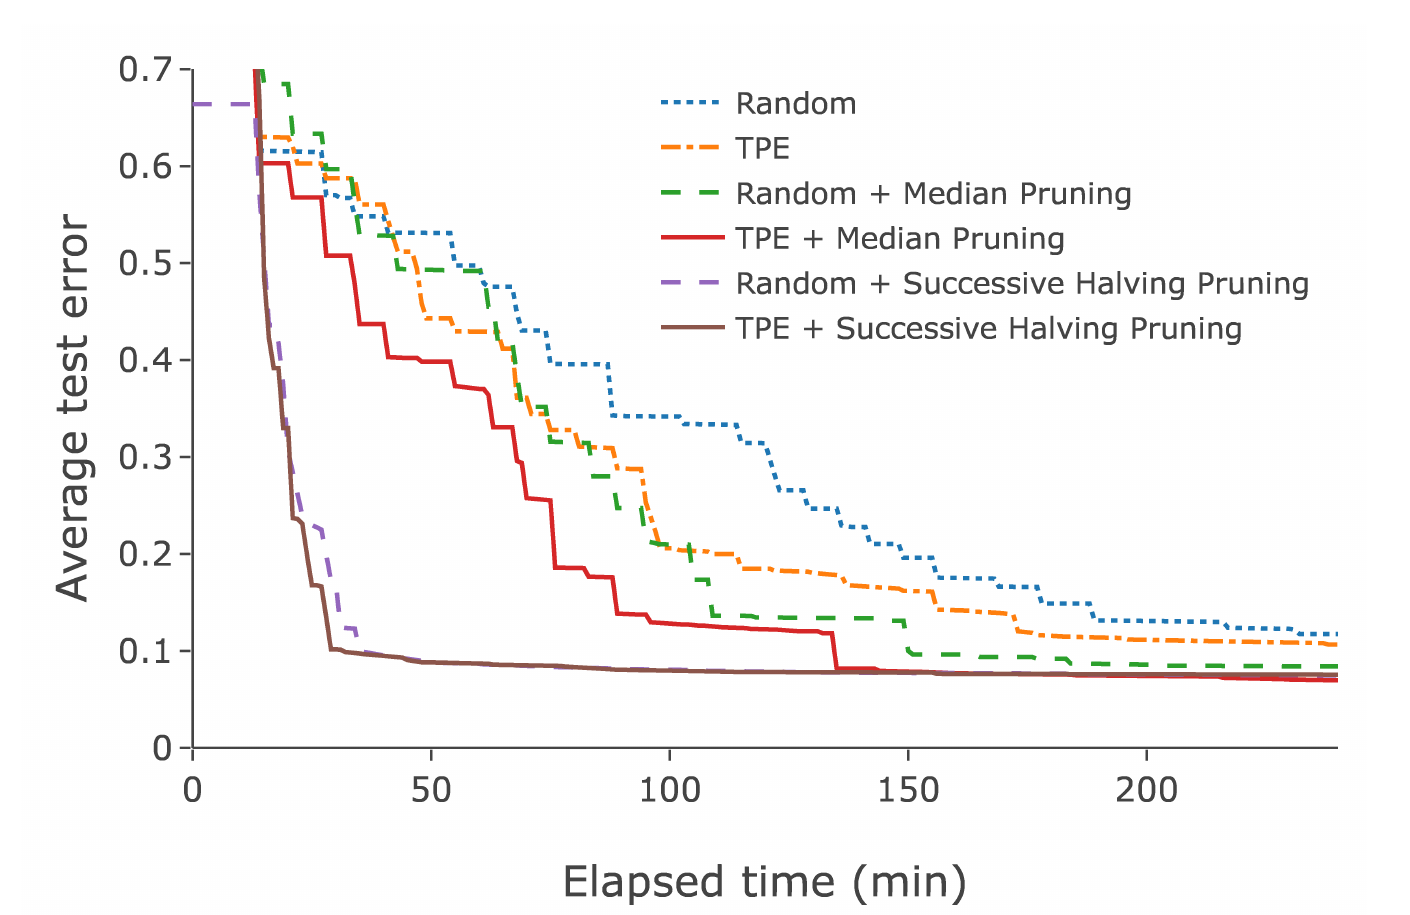
\includegraphics[width=0.62\textwidth,height=0.42\textheight,keepaspectratio]{images/mlops-foundations/optuna_pruning_test_error.png}

    {\scriptsize Source: Akiba, Sano, Yanase, Ohta \& Koyama, ``Optuna: A Next-generation Hyperparameter Optimization
    Framework,'' KDD 2019, \href{https://arxiv.org/abs/1907.10902v1}{arXiv:1907.10902v1}, Figure~11(a).
    Simplified AlexNet on SVHN; average test error against \emph{wall-clock} time.}

    \vspace{0.5em}
    \begin{itemize}
        \small
        \item Read the $x$-axis carefully: this is error against \textbf{elapsed time}, not against number of
              trials. That is the axis that costs money.
        \item TPE beats random search at equal time --- but the two curves that collapse almost immediately
              are the \textbf{pruned} ones. Pruning is the bigger win.
        \item In the same paper's RocksDB case study, a 4-hour budget explored \textbf{937} configurations
              with pruning versus \textbf{39} without.
    \end{itemize}

\end{frame}

% --- SLIDE 7: SEARCH SPACE + WHEN NOT TO ---
\begin{frame}{Search-Space Design, and When HPO Is Wasted Compute}

    \begin{columns}[T]
        \begin{column}{0.48\textwidth}
            \begin{tcolorbox}[colback=green!5, colframe=green!50!black, title=\scriptsize Designing the space]
                \scriptsize
                \begin{itemize}
                    \item \textbf{Few parameters, wide ranges} beats many parameters with narrow ones.
                    \item Log scale for anything multiplicative.
                    \item Bound the space with physics and budget, not superstition: if a depth of 40 will not
                          fit in memory, do not offer it.
                    \item If the best value sits on a \textbf{boundary}, your range was wrong --- widen it and
                          rerun.
                    \item Tune the \emph{pipeline}, not only the model: imputation strategy and scaler often
                          matter more than \texttt{n\_estimators}.
                \end{itemize}
            \end{tcolorbox}
        \end{column}
        \begin{column}{0.48\textwidth}
            \begin{tcolorbox}[colback=red!5, colframe=red!50, title=\scriptsize When to skip HPO entirely]
                \scriptsize
                \begin{itemize}
                    \item \textbf{The baseline is not built yet.} Tune nothing until a dumb model is logged.
                    \item \textbf{The validation set is small.} With 200 samples, 500 trials just find the
                          configuration that best overfits your split.
                    \item \textbf{The gain is not decision-relevant.} $+0.3$ F1 points that change no
                          business action is compute set on fire.
                    \item \textbf{The data is the bottleneck.} A week of labelling usually beats a week of
                          tuning.
                \end{itemize}
            \end{tcolorbox}
        \end{column}
    \end{columns}

    \vspace{0.15em}
    \begin{alertblock}{Guard the test set}
        The HPO objective must be computed on \textbf{validation} data --- ideally cross-validated. A search
        of 500 trials against a single small split is a very efficient overfitting machine.
    \end{alertblock}

\end{frame}
